\chapter{Differential expression analysis of tail loss in an invertebrate chordate}

\section{Introduction}

Chordates are composed of three subphyla\textemdash vertebra, tunicata and cephalochordata\textemdash that all share several characteristics, with the notochord being the key characteristic (from which the phylum name comes). The tail development of larvaceans such as Oikopleura dioica and several species of ascidians and tunicates has been well studied \cite{jeffery_factors_1992,nakatani_mutations_1999,kugler_evolutionary_2011}. Larvaceans form tailed larvae with a hollow dorsal notochord and keep their tail throughout their adult life stage. Ascidians generally form their tail in a similar manner before undergoing the process of metamorphosis, in which the larval tail is absorbed in to the trunk region \cite{paris_history_2008}. A typical ascidian larvae tail forms through the convergence, intercalation and extension of the notochord and the differentiation of the posterior muscle cells \cite{swalla_mechanisms_1993}. When fully formed the ascidian notochord contains 40 cells, flanked by three rows of muscle cells. The ancestral notochord or notochord-like structure is believed to have been muscle based, which is perhaps the reason that the tail formation is often contingent upon proper development of both notochord and muscles \cite{lauri_development_2014}. This idea is supported by the observation that the primary and secondary notochord and muscle lineage are derived from the same blastomere, and the ascidian tail needs both the notochord and differentiated muscle to form a larval tail \cite{nishida_cell_1987,di_gregorio_tail_2002}.

Of the \mytilde3000 species of ascidians fewer than 20 do not form a tail, with the majority being Molgulidae species \cite{berrill_studies_1931,huber_evolution_2000}. This likely represents several independent instances of evolutionary loss of the tail, and introduces the question of why are the Molgulidae so susepectibale to tail-loss. Although the mechanism behind tail-loss differs by species, a common characteristic is the lack of a notochord that intercalates and extends, as well as a less differentiated central nervous system (CNS) structures and tail muscles \cite{swalla_mechanisms_1993}. \textit{Molgula bleizi} notochord cells converge to the midline, and began to extend, but cells never properly intercalate and the tail formation stops before it is fully formed \cite{jeffery_evolution_1999}. In \textit{M. bleizi} there is an early down-regulation of \textit{brachyury} (\textit{bra})\textemdash a key notochord inducer\textemdash and larva-specific muscle actin genes have become pseudo genes.   

A similar situation is observed in \textit{Molgula occulta}: muscle actins have become pseudogenes, independently of their conversion in \textit{M. bleizi}. \textit{M. occulta} and \textit{Molgula oculata} are two closely related species, who in their adult form are virtually identical, with the exception of a white pigment spot between the two siphons of the tailed species, \textit{M. oculata}. During development the species are indistinguishable up to the gastrula stage. In late gastrula when the notochord and muscle progenitors begin to move posteriorly \cite{swalla_novel_1993} and the notochord begins to form, the morphological divergence becomes evident. Through subtractive screening Swalla and Jeffery \cite{swalla_requirement_1996} have identified \textit{manx}, a zinc finger transcription factor (TF) and the cytoskeletal protein p58 to be down-regulated in \textit{M. occulta} relative to \textit{M. oculata} \cite{swalla_identification_1991}, amongst other genes were shown to be one of the causes of the tail loss in \textit{M. occulta}. There are several steps that take place to form the notochord and tail: first, the notochord cells move mediolaterally to the midline; and next, the cells polarize and intercalate, changing their shape and extending posteriorly \cite{keller_mechanisms_2000, jiang_ascidian_2005,stemple_structure_2005}. This process is known as convergence and extension. Although the two species have different developmental programs, crossing the tail-less \textit{M. occulta} eggs with sperm of the tailed \textit{M. oculata} produces a hybrid with 20 notochord cells like the tail-less species, but in which the cells intercalate and extend like the tailed species. In the hybrids the expression of \textit{manx} and p58 are restored, and antisense phosphorothiated oligodeoxynucleotide \textit{manx} in the hybrids have shown that zygotic \textit{manx} is necessary for tail formation \cite{swalla_requirement_1996}.

Several key tail development genes have been identified as present in the \textit{M. occulta} genome, but expressed at low levels during embryogenesis \cite{swalla_interspecific_1990,jeffery_factors_1992,swalla_novel_1993}. When expressed, some of these genes were shown to restore features in the hybrid. With advances in high throughput sequencing technologies, gene expression of \textit{M. occulta}, \textit{M. oculata}, and hybrid species can be analyzed on a whole transcriptome level \cite{gyoja_analysis_2007,pickrell_variation_2010}. mRNA of three different developmental stages for \textit{M. occulta}, \textit{M. oculata}, and their hybrid has been sequenced and assembled at Michigan State University (MSU). These three transcriptomes were used to% identify the presence or absence 
assess the expression levels of known notochord genes downstream of \textit{bra} using \textit{C. intestinalis} data from the NCBI database (\url{ncbi.nlm.nih.gov}). BLAST searches were done against known notochord genes, and several of them were selected for further analysis, including \textit{FGF9/16/20}, \textit{prickle (pk)}, and several other downstream genes.  These genes were then used to construct a putative \textit{brachyury} gene regulatory network for both \textit{M. occulta} and \textit{M. oculata}. 

\section{Methods}
\subsection{Sample collection, sequencing and assembly}
RNA was extracted from all three \textit{Molgula} species using the methods discussed in Lowe et al. \cite{lowe_evaluating_2014}. RNAs for the gastrula (3hpf), neurula (4hpf) and mid-tailbud (6hpf) stages were extracted for both \textit{M. occulta} and \textit{M. oculata}, with a replicate for the gastrula and a sample for early-tailbud stage sequenced from \textit{M. occulta}. %Samples from a fertilized embryo, tailbud and larvae were sequenced for \textit{M. occidentalis} to gain a broad scope of expression.
DNA was extracted from the gonads of an individual adult specimen for %\textit{M. occidentalis},
\textit{M. occulta}, and \textit{M. oculata}. Two paired-end jumping libraries were collected for each species ranging from \mytilde300bp to \mytilde950bp. Further details about extraction methods and libraries can be found in Stolfi et al., \cite{stolfi_divergent_2014}. Sequencing for \textit{M. occulta} and \textit{M. oculata} RNA were conducted at the Michigan State University, while all other sequencing was done at New York University. All libraries were paired-end, with 75 base pair (bp) reads for the sequencing done at MSU and 100 bp reads for the NYU sequencing. 

Genome assemblies were conducted using 3-pass digital normalization \cite{brown_reference-free_2012} and assembled using Velvet\cite{zerbino_velvet:_2008}. Other assemblers were tested, however, Velvet produced the best results with the least fragmented assemblies. Assemblies were initially done with 21 $\geq$ k $\geq$ 71, for intervals of 10. We selected the 'k' value with the highest N50, and then the genomes were reassembled for a k$\pm$10 with a step size of 2 for the selected assembly, and the best N50 was chosen. A k of 31, and 49 were select for \textit{M. occulta}, and \textit{M. oculata}, respectively. 

Both \textit{de novo} and reference based assemblies were used to create gene models. Reads were mapped to their respective genomes using bowtie2 and tophat to identify genes and alternative splicing variants \cite{langmead_fast_2012,trapnell_differential_2012}. The accepted.bam files were then sorted and indexed using samtools \cite{li_sequence_2009}. The sorted bam files were then processed using cufflinks and cuffmerge to generated consensus gtf annotation files. The digitally normalized trinity \textit{de novo} assembled transcripts from Lowe et al. \cite{lowe_evaluating_2014}, were aligned to their respective genomes using BLAT \cite{haas_novo_2013}. The cufflinks/cuffmerged gtf files were then converted into bed files and merged with the annotation files from the mapped \textit{de novo} assembly aligned using gimme (\url{https://github.com/likit/gimme}). Gimme joins gene models using a graph based method to develop more complete transcripts. The gimme gene models were then converted to gff format using the script bed2gff in the gimme utils folder in order to extract the transcripts from the genome in a multi fast file. Transcripts were then extracted using ``gffread -w transcripts.fa -g /path/to/genome.fa transcripts.gtf'' which is included in the cufflinks package. The extracted transcripts were partitioned into transcript families and annotated using the khmer suite and steps found in the eel-pond protocol (\url{https://khmer-protocols.readthedocs.org/en/latest/mrnaseq/index.html}). \textit{Ciona intestinalis} was used as an annotation reference, and the sequences were retrieved as discussed in Chapter 3. 

\subsection{Gene counts and differential expression analysis}
Reads were mapped to transcripts from the gimme gene models for their respective species. Reads from the hybrids were mapped onto both the \textit{M. occulta} and \textit{M. oculata} transcripts, since the hybrids are F1 hybrids and should contain an allele from each parent. Read counts were generated using eXpress \cite{roberts_streaming_2013}. eXpress gives the option of ``Total counts'' and ``Effective counts'', which reports the number of reads mapped per transcript and the normalized counts based on transcript length, respectively. Because EdgeR uses unnormalized reads, ``Total counts'' were used. Counts for hybrid reads mapped to \textit{M. occulta} and \textit{M. oculata} were combined to calculate total expression at a given stage. A replicate was only provided for one of the samples, 3hpf, and because of this 5hpf was treated as a replicate for 6hpf. These time points correspond to early and mid-tail bud stages in the tailed ascidian. 

Differential expression was calculated using the Bioconductor EdgeR package because of its ability to work with minimal replicates \cite{robinson_edger:_2010}. We ran RBH  for \textit{M. occulta} and \textit{M. oculata} in order to identify orthologous transcripts to conduct allele specific differential expression analysis on the hybrid. We used both estimateGLMCommonDisp and estimateGLMTagwiseDisp to calculate dispersions. There is only a replicate for \textit{M. occulta} gastrula stage (F+3), because of this we used \textit{M. occulta} early tailbud stage as a replicate for the mid tailbud stage. These replicates were used to calculate dispersions for all samples. Exact-test with p = 0.05 were used for differential expression, and transcripts with false discovery rate (FDR) of 0.05 being called as differentially expressed. 

\section{Results}
\subsection{\textit{M. occulta} and \textit{M. oculata} have strong overlap in gene expression}
\textit{C. intestinalis} is the closest ascidian species with a well annotated genome, and so we used \textit{Ciona} proteins obtained from the NCBI to annotate the genomes of both \textit{M. occulta} and \textit{M. oculata}. Reciprocal best hit (RBH) blast with an e-value of 1e-3, were done with the \textit{M. occulta} and \textit{M. oculata} transcriptomes against \textit{C. intestinalis} for the annotation of both \textit{Molgula} species.  We are aware this is a low threshold for homology, however, information for these species are not known and we wanted to gain as much insight as possible for genes and gene function. Moreover, the reciprocal best hit criterion is extremely stringent.

The gene models for \textit{M. occulta} and \textit{M. oculata} produced 42,365 and 40,775 sequences total, respectively. Precisely 8,627 \textit{M. occulta} transcripts were annotated as orthologs and 22,700 transcripts were annotated as showing homology. Similar annotation numbers were produced with \textit{M. oculata}: 8,677 showed orthology, and 22,583 showed homology. \textit{M. occulta} and \textit{M. oculata} have a high overlap in number of translated transcripts that showed any level of homology with \textit{C. intestinalis} proteins from the NCBI database. Of the 16,414 {\em Ciona} proteins, \textit{M. occulta} had BLAST hits for 83.6\% and 86.5\% had hits in \textit{M. oculata}. \textit{M. occulta} had hits for 453 proteins that were not found in \textit{M. oculata} and \textit{M. oculata} had hits for 921 transcripts that did not have hits in \textit{M. occulta}, yielding an overlap of 97\% in assembled homologs.

\begin{figure}[tbp]
\centering
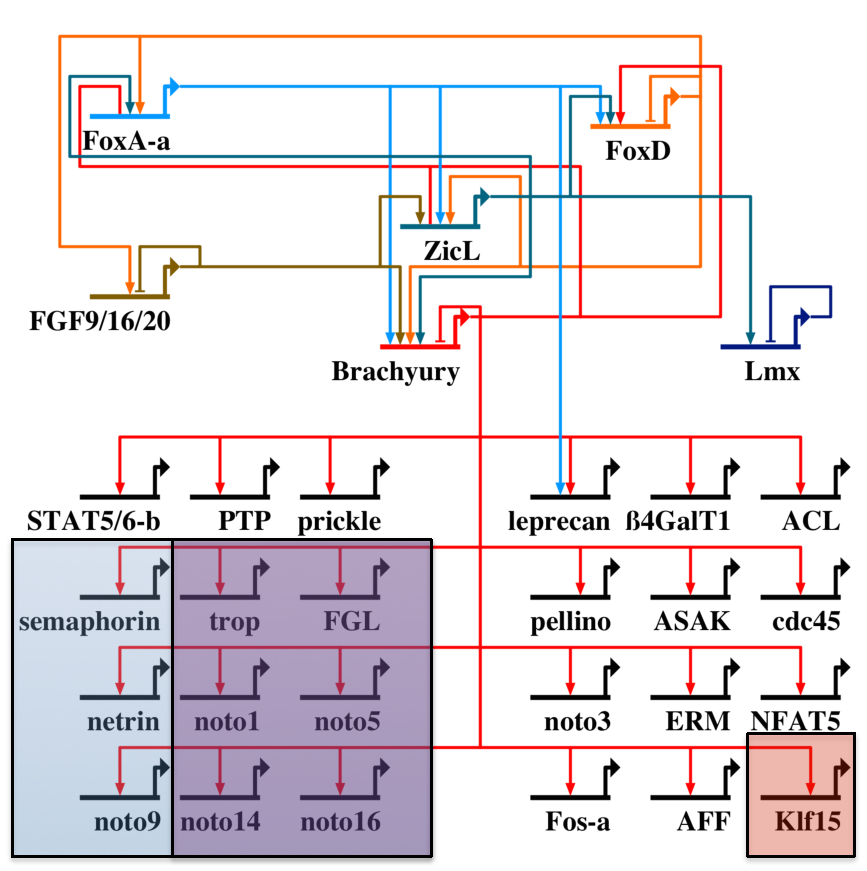
\includegraphics[scale=0.8]{figures/bra_grn.pdf}
\caption{\textbf{\textit{Brachyury gene regulatory network.}}\textit{Bra} is a key notochord inducer, and without its expression neither the notochord nor the chordate tail forms. Downstream genes have been identified in various studies and of these 67 genes 11 were missing from the transcriptomes of both species. The missing genes were \textit{cofilin}, \textit{entactin} (\textit{nidogen-2-like}), \textit{fibrinogen-like protein} (\textit{FGL}), \textit{fibronectin}, \textit{multidom}, \textit{noto1}, \textit{noto5}, \textit{noto14}, \textit{noto16}, and \textit{tropomyosin}. \textit{netrin}, and \textit{noto9} are missing in \textit{M. occulta} and \textit{Klf15} is missing in \textit{M. oculata}. (Blue) missing in \textit{M. occulta}, (Red) missing in \textit{M. oculata}, and (Purple) missing in both species. This GRN was built from previous studies  \cite{hotta_temporal_1999,hotta_characterization_2000,hotta_brachyury-downstream_2007,kugler_evolutionary_2008,kugler_evolutionary_2011}, using the BioTapestry software \cite{longabaugh_visualization_2009}.}
\label{fig:bra_grn}
\end{figure}
\subsection{Notochord gene network}

Next, we examined genes associated with notochord development in \textit{C. intestinalis} to investigate the molecular development of the tail. Gene candidates were identified as being involved in tail formation and notochord development through previous analysis of genes downstream of \textit{bra} \cite{hotta_temporal_1999,hotta_characterization_2000,hotta_brachyury-downstream_2007,kugler_evolutionary_2008,kugler_evolutionary_2011}. From these studies many potential notochord genes were identified; we compiled a list of 67 genes and identified those expressed during the gastrula, neurula or tailbud stages within the %genomes and 
transcriptomes of both \textit{M. occulta} and \textit{M. oculata} (Figure~\ref{fig:bra_grn}). Of the 67 genes, 11 were not expressed in the transcriptomes of either species: \textit{cofilin}, \textit{entactin} (\textit{nidogen-2-like}), \textit{fibrinogen-like protein} (\textit{FGL}), \textit{fibronectin}, \textit{multidom}, \textit{noto1}, \textit{noto5}, \textit{noto14}, \textit{noto16}, and \textit{tropomyosin}. The remaining genes without orthologous sequences were \textit{netrin}, and \textit{noto9} in \textit{M. occulta} and \textit{Klf15} in \textit{M. oculata}. In \textit{Ciona}, \textit{netrin} is expressed in the notochord and the central nervous system and is associated with axon guidance \cite{hotta_characterization_2000}. \textit{Klf15} was detected in the notochord, but there is currently no known information regarding its function \cite{passamaneck_direct_2009}. Taken together, these demonstrates a strong overlap in the presence of the number of genes associated in notochord formation in both \textit{M. occulta} and \textit{M. oculata}.

\subsection{Differential expression between neurula and tailbud appears to be key factor in tail development} 

\begin{table}[b]
\caption{Differential expression: Species \textit{vs} time}
\makebox[\linewidth]{
\centering
\begin{tabular}{l c c c c}
\hline\hline
{\multirow{2}{*}{Species} } & {\multirow{2}{*}{Condition} }&\multicolumn{3}{c}{Number of transcripts that show...} \\ %\cline{1-6}% inserts table %heading
& & Up-regulation & Down-regulation & No differential expression \\ [0.5ex]
\hline
{\multirow{2}{*}{\textit{M. occulta} }} 	&						
from Gastrula to Neurula& 260 & 8 & 20197  \\ 
\multicolumn{1}{ l  }{}                        			&				
from Neurula to Tailbud&1 & 4 & 20460    \\ \cline{1-5}
{\multirow{2}{*}{\textit{M. oculata} }} &
from Gastrula to Neurula& 119 & 66 & 20280  \\ 
\multicolumn{1}{ c  }{}                        &
from Neurula to Tailbud&1170 & 626 & 18669    \\ \cline{1-5}
{\multirow{2}{*}{Hybrid }} &
from Gastrula to Neurula& 21 & 99 & 20345  \\ 
\multicolumn{1}{ c  }{}                        &
from Neurula to Tailbud&1270 & 129 & 19066    \\ 
\hline
\end{tabular}
\label{table:de}
}
\end{table}

\begin{landscape}
\begin{figure}[!H]
	\subfloat[\label{subfig:mocc3v4}]{%
	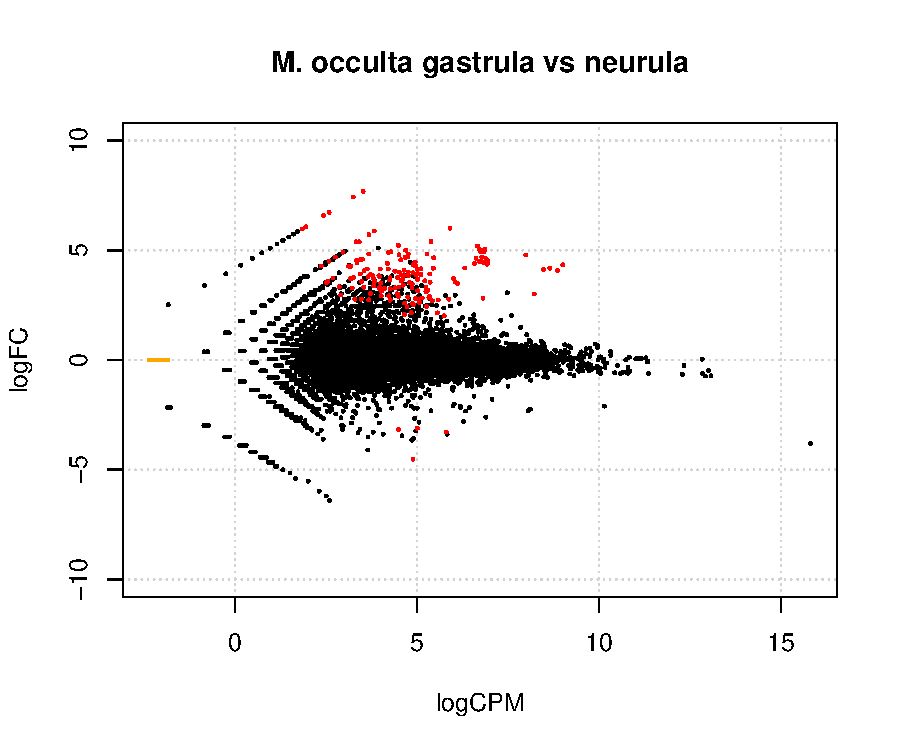
\includegraphics[scale=0.45]{figures/mocc3v4_graph.pdf}
	}
	\subfloat[\label{subfig:mocu3v4}]{%
	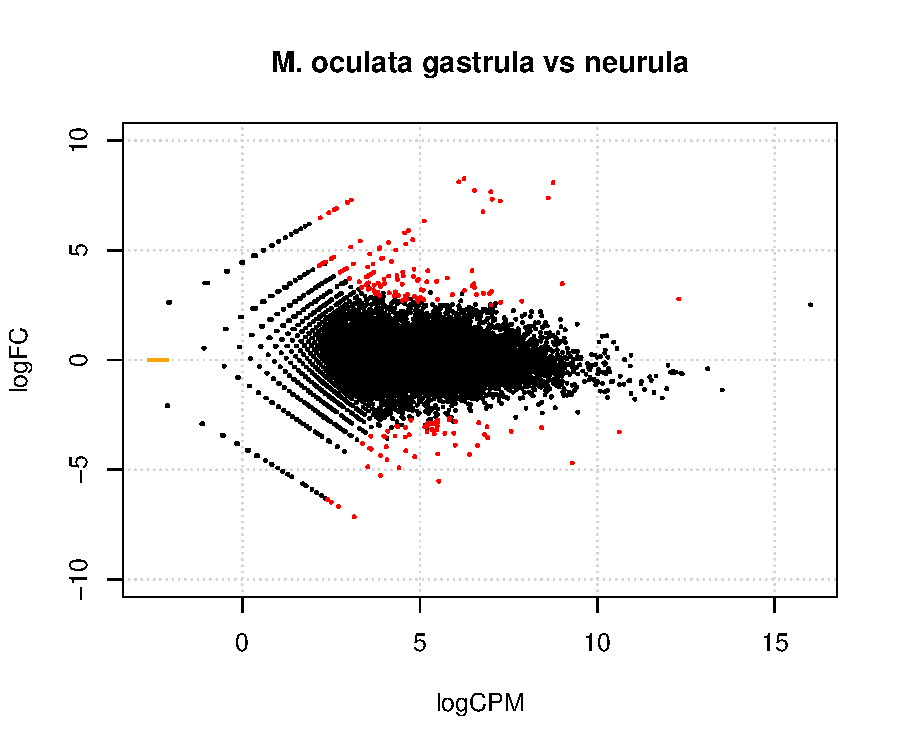
\includegraphics[scale=0.45]{figures/mocu3v4_graph.pdf}
	}
	\subfloat[\label{subfig:hyb3v4}]{%
	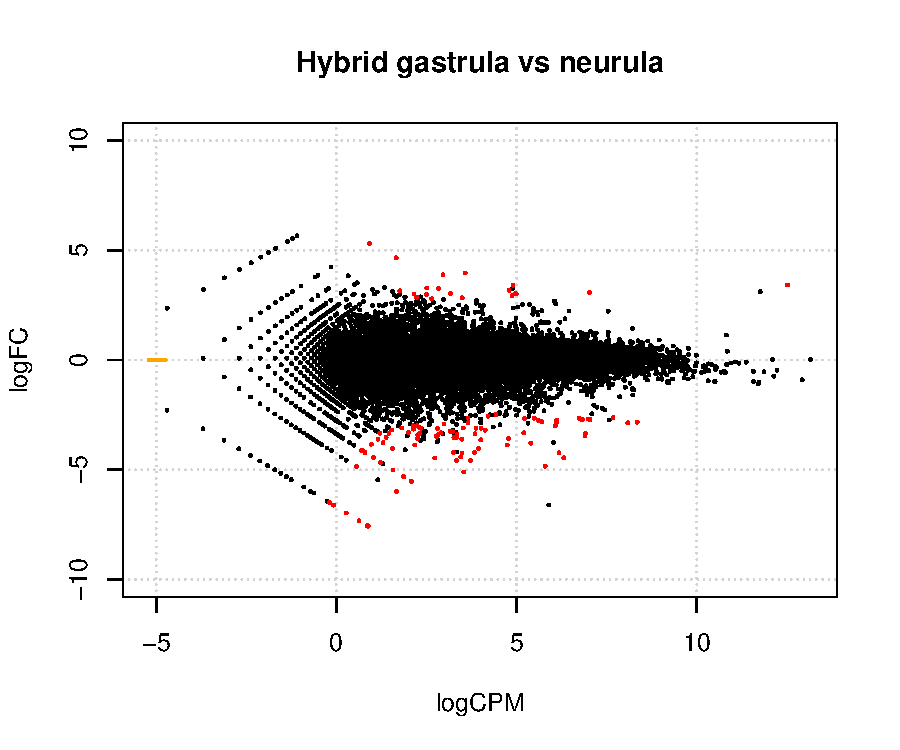
\includegraphics[scale=0.45]{figures/hyb3v4_graph.pdf}
	}
	\hfill
	\subfloat[\label{subfig:mocc4v6}]{%
	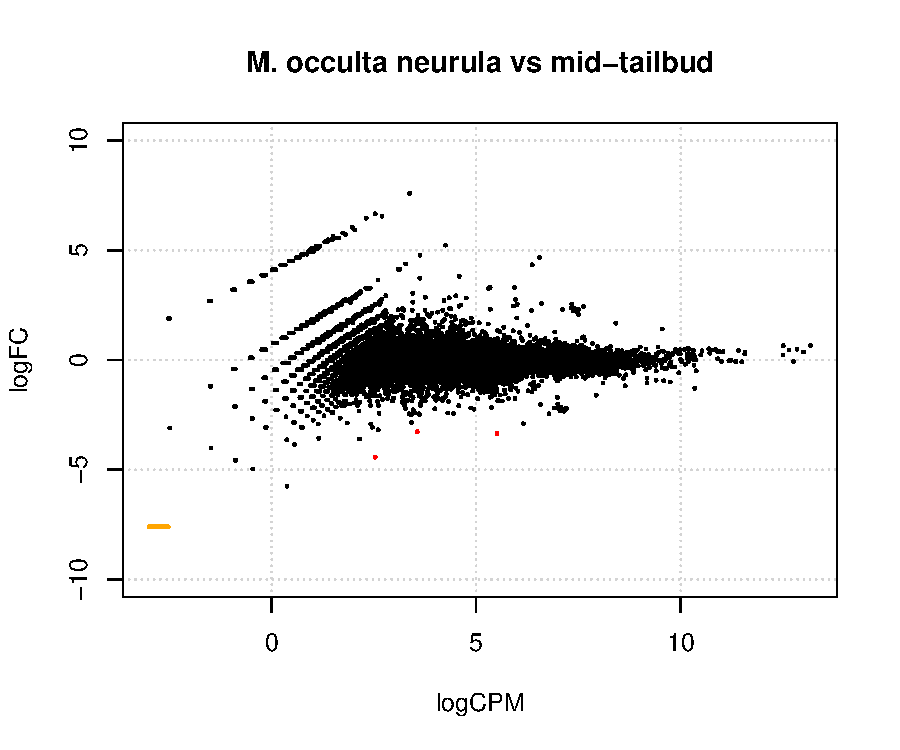
\includegraphics[scale=0.45]{figures/mocc4v6_graph.pdf}
	}
	\subfloat[\label{subfig:mocu4v6}]{%
	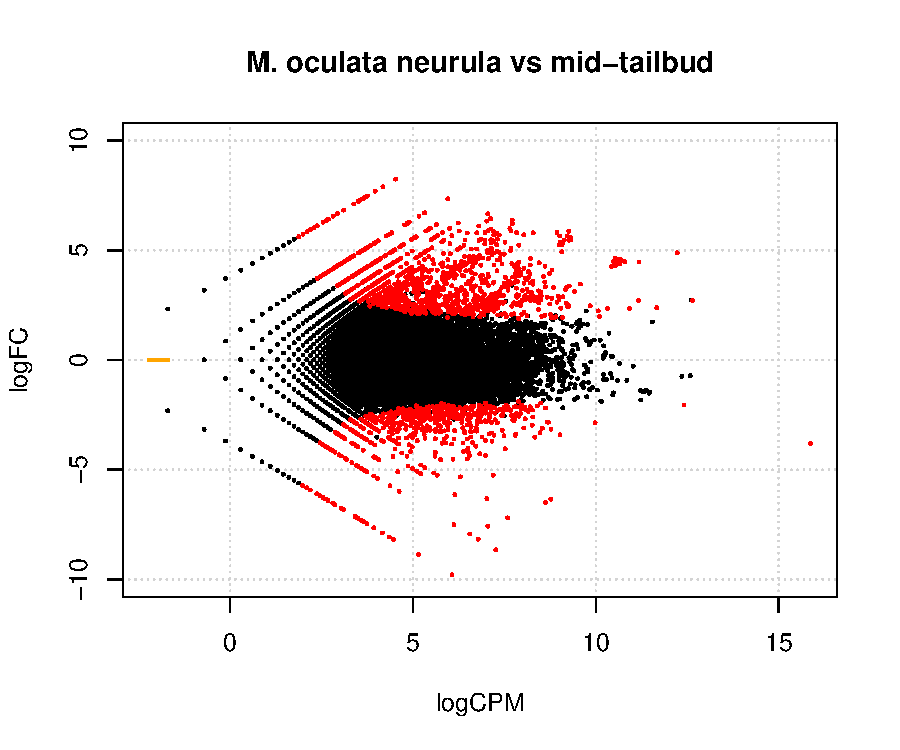
\includegraphics[scale=0.45]{figures/mocu4v6_graph.pdf}
	}
	\subfloat[\label{subfig:hyb4v6}]{%
	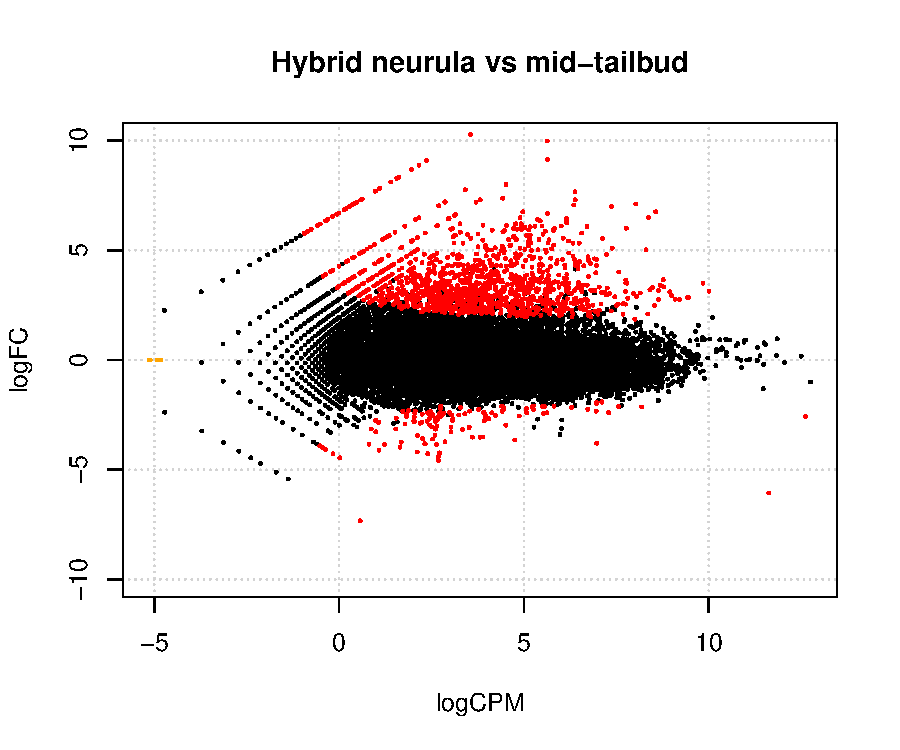
\includegraphics[scale=0.45]{figures/hyb4v6_graph.pdf}
	}
	\caption{\textbf{Differential expression of homologous transcripts.} Differential expression in \textit{M. occulta} for (a) gastrula vs neurula, and (d) neurula vs tailbud, \textit{M. oculata} for (b) gastrula vs neurula, and (e) neurula vs tailbud, and the hybrid for (c) gastrula vs neurula, and (f) neurula vs tailbud. Genes in red are differentially expressed with a FDR \textless 0.05}
	\label{fig:de_plots}
\end{figure}
\end{landscape}

Only in \textit{M. occulta} embryos that expressed \textit{manx} and p58 produced hybrids with urodele features. To identify other candidate genes whose differential expression in \textit{M. occulta} may contribute to the tail-less condition, we sequenced and assembled three developmental stages\textemdash gastrula, neurula, and tailbud\textemdash across \textit{M. occulta}, \textit{M. oculata} and their interspecies hybrid. The tail-less species, \textit{M. occulta}, showed the highest level of differential expression (FDR \textless 0.05), with 260 (97\%) of the identified differentially expressed transcripts being up-regulated in the neurula stage relative to the gastrula stage. (Table~\ref{table:de}). \textit{M. oculata} also had more transcripts being up-regulated (65\%) than down at the neurula stage relative to the gastrula. Hybrids did not follow this trend; the majority of its genes are down-regulated (82\%).  

When comparing the tailbud stage to the neurula stage there was essentially no significant differential expression observed in \textit{M. occulta}. A total of 5 genes were said to be differentially expressed (FDR \textless 0.05). However a major shift in differential expression was seen in both \textit{M. oculata} and the hybrid at the tailbud stage relative to the neurula stage (Figure~\ref{fig:de_plots}). There were 1170 and 1270 transcripts up-regulated, and transcripts and 129 transcripts down-regulated in \textit{M. oculata} and the hybrid respectively. That equates to a 10\textit{x} increase in differentially expressed transcripts in both hybrid and \textit{M. oculata} tailbud embryos relative to the respective neurula stage embryos..

\subsection{Overlap between hybrid and M. oculata alleles}
When comparing transcript expression from neurula to tailbud in \textit{M. oculata} and the hybrid there is a total of 2,440 transcripts up-regulated collectively. Of these 2,440 transcripts, 328 (13\%) overlap (Figure~\ref{subfig-1:overlap}). There were no transcripts in \textit{M. occulta} identified as differentially expressed that overlapped with either \textit{M. oculata} or their hybrid. Of the transcripts that were down regulated, there was only an overlap of 5 transcripts (0.06\%) between \textit{M. oculata} and the hybrid, and again none between \textit{M. occulta}. To take a closer look at these dynamically regulated transcripts, we examined their allele specific expression to determine if the \textit{M. oculata} alleles represented the majority of this gene expression in the hybrids, or if there was some rescue of expression of the \textit{M. occulta} alleles. When analyzing the 328 up-regulated transcripts that overlapped between \textit{M. oculata} and the hybrid, there was large skew for expression from the \textit{M. oculata} allele: 91.7\% of expression came from \textit{M. oculata} (Figure~\ref{subfig-2:overlap_allele}). A similar but far less dramatic trend was observed for the transcripts up-regulated in hybrid but not overlapping with \textit{M. oculata}, with more expression coming from the \textit{M. oculata} allele. The allele specific differential expression at tailbud was 32\% \textit{M. oculata}, 36\% \textit{M. occulta} and 32\% hybrid.

\begin{figure}[!ht]
	\subfloat[\label{subfig-1:overlap}]{%
	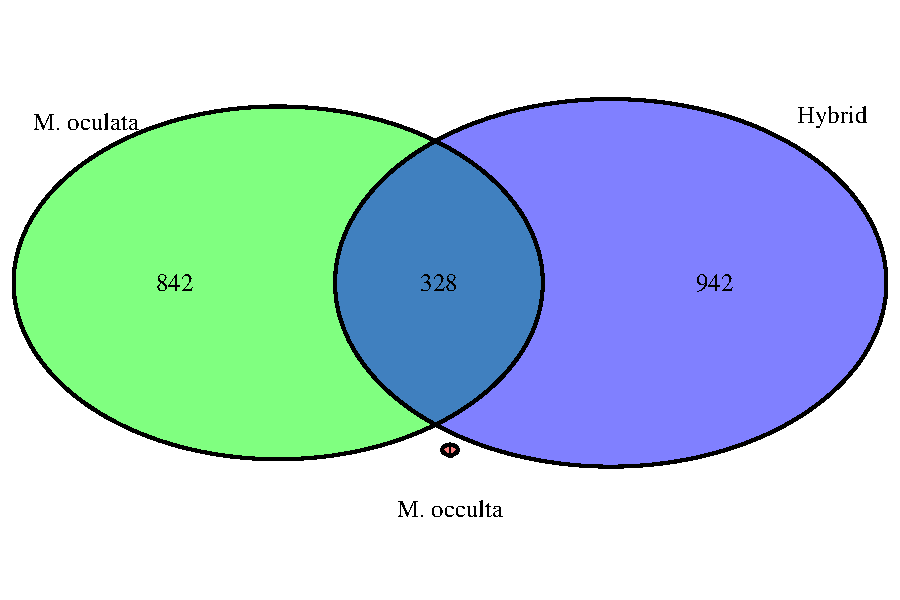
\includegraphics[width=0.45\textwidth]{figures/up_reg.pdf}
	}
	\subfloat[\label{subfig-2:overlap_allele}]{%
	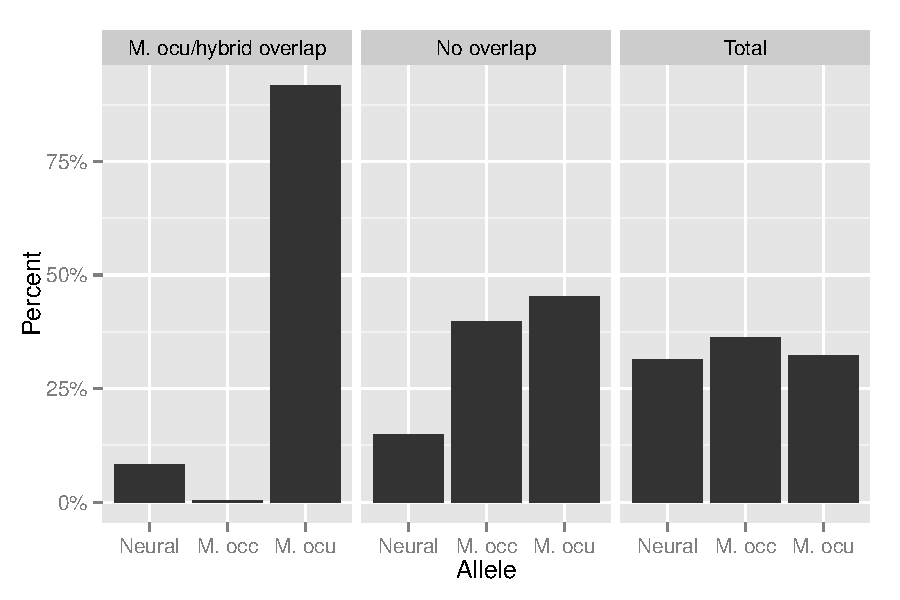
\includegraphics[width=0.45\textwidth]{figures/up_reg_allele_tb.pdf}
	}
	\caption{\textbf{Upregulated transcripts overlap between hybrid and \textit{M. oculata}.} When comparing the gastrula and neurula time point for \textit{M. occulta}, \textit{M. oculata}, and their hybrid, both \textit{M. oculata} and the hybrid showed differential expression in at least 7\% of their transcripts with the majority being up-regulated. (\ref{subfig-1:overlap}) There is a 15\% overlap in overexpressed genes \textit{M. oculata} and the hybrid, for the transcripts overexpressed when comparing gastrula to neural expression, and there is no overlap with \textit{M. occulta}. (\ref{subfig-2:overlap_allele}) When looking at the allelic express for the same condition, there is a strong skew in expression coming from the tailed allele for the unregulated transcripts that overlap between \textit{M. oculata} and the hybrid. The highest percentage of transcripts of allelic expression in the hybrid also comes from \textit{M. oculata} for up-regulated transcripts that do not overlap with \textit{M. oculata}, but not to as great an effect.  For genes' overall allelic expression, the majority comes from \textit{M. occulta}, 36\%, with 32\% coming from \textit{M. oculata}.}	
	\label{fig:upreg_tb}
\end{figure}

\section{Discussion}
Several genes identified as expressed in the notochord of \textit{C. intestinalis} \cite{hotta_characterization_2000,hotta_brachyury-downstream_2007} were observed to be missing in both \textit{M. occulta} and \textit{M. oculata}; of these genes all were also identified as being missing in the \textit{O. dioica} \cite{kugler_evolutionary_2011}. The lack of expression of these gene is the Molgulids and \textit{O. dioica} implies these genes are not necessary for the development of a fully functional notochord, CNS, or muscles in the ancestral chordate and are specific for \textit{Ciona}.

Here we present a differential expression analysis of two closely related \textit{Molgula} species, \textit{M. occulta} and \textit{M. oculata}, using high throughput sequencing technology. We were able to create gene models using both a mapping based approach and \textit{de novo} assembly approach, and then combined the assemblies for better transcript models. We showed that from neurula to the tailbud stage there is a 10 fold increase in transcripts that are identified as differentially expressed (p=0.05) in both \textit{M. oculata} and the hybrid. Using this same condition we were able to show that there is almost no differential expression in the the tail-less \textit{M. occulta}. This result  correlate with the embryo morphologies during this transition; in \textit{M. oculata}, the processes of tail formation are occurring, which may explain the increased transcriptional activity. In contrast in \textit{M. occulta} there are no noticeable morphological changes occurring. In hybrid embryos, this dynamic regulation of gene expression at the tailbud stage is rescued. Because hybrids show partially rescued tails and CNS structures, I propose that these transcripts may have an important role in the formation of the tail. Furthermore, of those transcripts upregulated at the tailbud stage in the hybrid but not in \textit{M. occulta}, it appears that expression is being restored from the \textit{M. oculata} genome, the zygotic allele. This suggests that the relative lack of differential gene expression in the neurula-to-tailbud transition in \textit{M. occulta} may be due to loss-of-function of cis-regulatory elements controlling the expression of key genes involved in tail and CNS formation. 

\section{Conclusion}

We have used two closely related Molgulids with the ability to hybridize to study three key time points in tail development: gastrulation, neurulation and tailbud. This study has shown that from neurula to tailbud number of transcripts are up-regulated, in both \textit{M. oculata} and the hybrid. Not only are transcripts up-regulated in this condition, with no significant differential expression in the tail-less species, but there is also an overlap between the differentially expressed genes in the \textit{M. oculata} and the hybrid. Seeing that both \textit{M. occulta} and \textit{M. oculata} have a strong overlap in genes identified to be involved in notochord develop, this differential expression could be the possible cause of loss of the tail and notochord and CNS in \textit{M. occulta}. 

The hybrids shed light on the fact that cis-regulatory elements are one of the key causes for the lack of urodele features in the tai-less \textit{M. occulta}. Previously, it has been shown that \textit{Molgula} have a high turnover in sequences of cis-regulatory elements, diverging is binding sites, while keeping the orthologous gene expression \cite{}. Perhaps, this cis-regulatory turnover has also led to the (turning of of these sites, i can't think of a smart way to say it, I'm running on fumes). 
